\chapter{Concept}
\label{ch:concept}

This chapter introduces the main concept of our research.
Section~\ref{sec:Identifying case studies and actions} describes the theory that helps us
to come up with the case-studies and the possible interactions of social devices.
Section~\ref{sec:Identifying personality traits} identifies the mascots' personality traits
that they will display during interactions described in previous section.
In Section~\ref{sec:Identifying the vibration level based on the personality traits},
based on the assigned personalities, we explore the possible actions
that social devices show while interacting with each other.
In Section~\ref{sec:Identifying the vibration level based on the personality traits},
we identify the vibration levels that convey personality traits.
In Section~\ref{sec:Identifying the music preferences based on the personality traits},
we associate the music genre with personality traits.
Section~\ref{sec:Identifying the color based on personality traits} describes
colors that convey mascots' personality traits.
Section~\ref{sec:overview-of-the-system-based-on-the-applied-concepts.} gives an overview of a system
based on the concepts described in the previous sections of this chapter.

\section{Identifying case studies and actions}
\label{sec:Identifying case studies and actions}

In our research, we extended the "Autonomous Cooperation of Social Things" ~\cite{okada2016autonomous}
by applying Proxemics Theory and Personality Traits Model.

Based on the Proxemics theory~\cite{hall1966hidden, hall1963system}, we classify our devices in the following way:
mascot will belong to the intimate, tablet to a personal,
lamp will be considered as a social and speakers as public distance.
In this way, these objects represent cooperation among these distances.
According to this theory, the distance between people represents their
relationship which affects the way how they interact with each other.
Having understood how people use distance when interacting with each other,
and then applying this concept to social devices, we can come up with four case studies:
mascot-mascot, mascot-tablet, mascot-lamp and mascot-speakers interactions.
Figure~\ref{fig:Proxemics} shows the visual representation of selected devices based on
four distances introduced by the theory of proxemics.
\begin{figure}[hbt!]
    \centering
    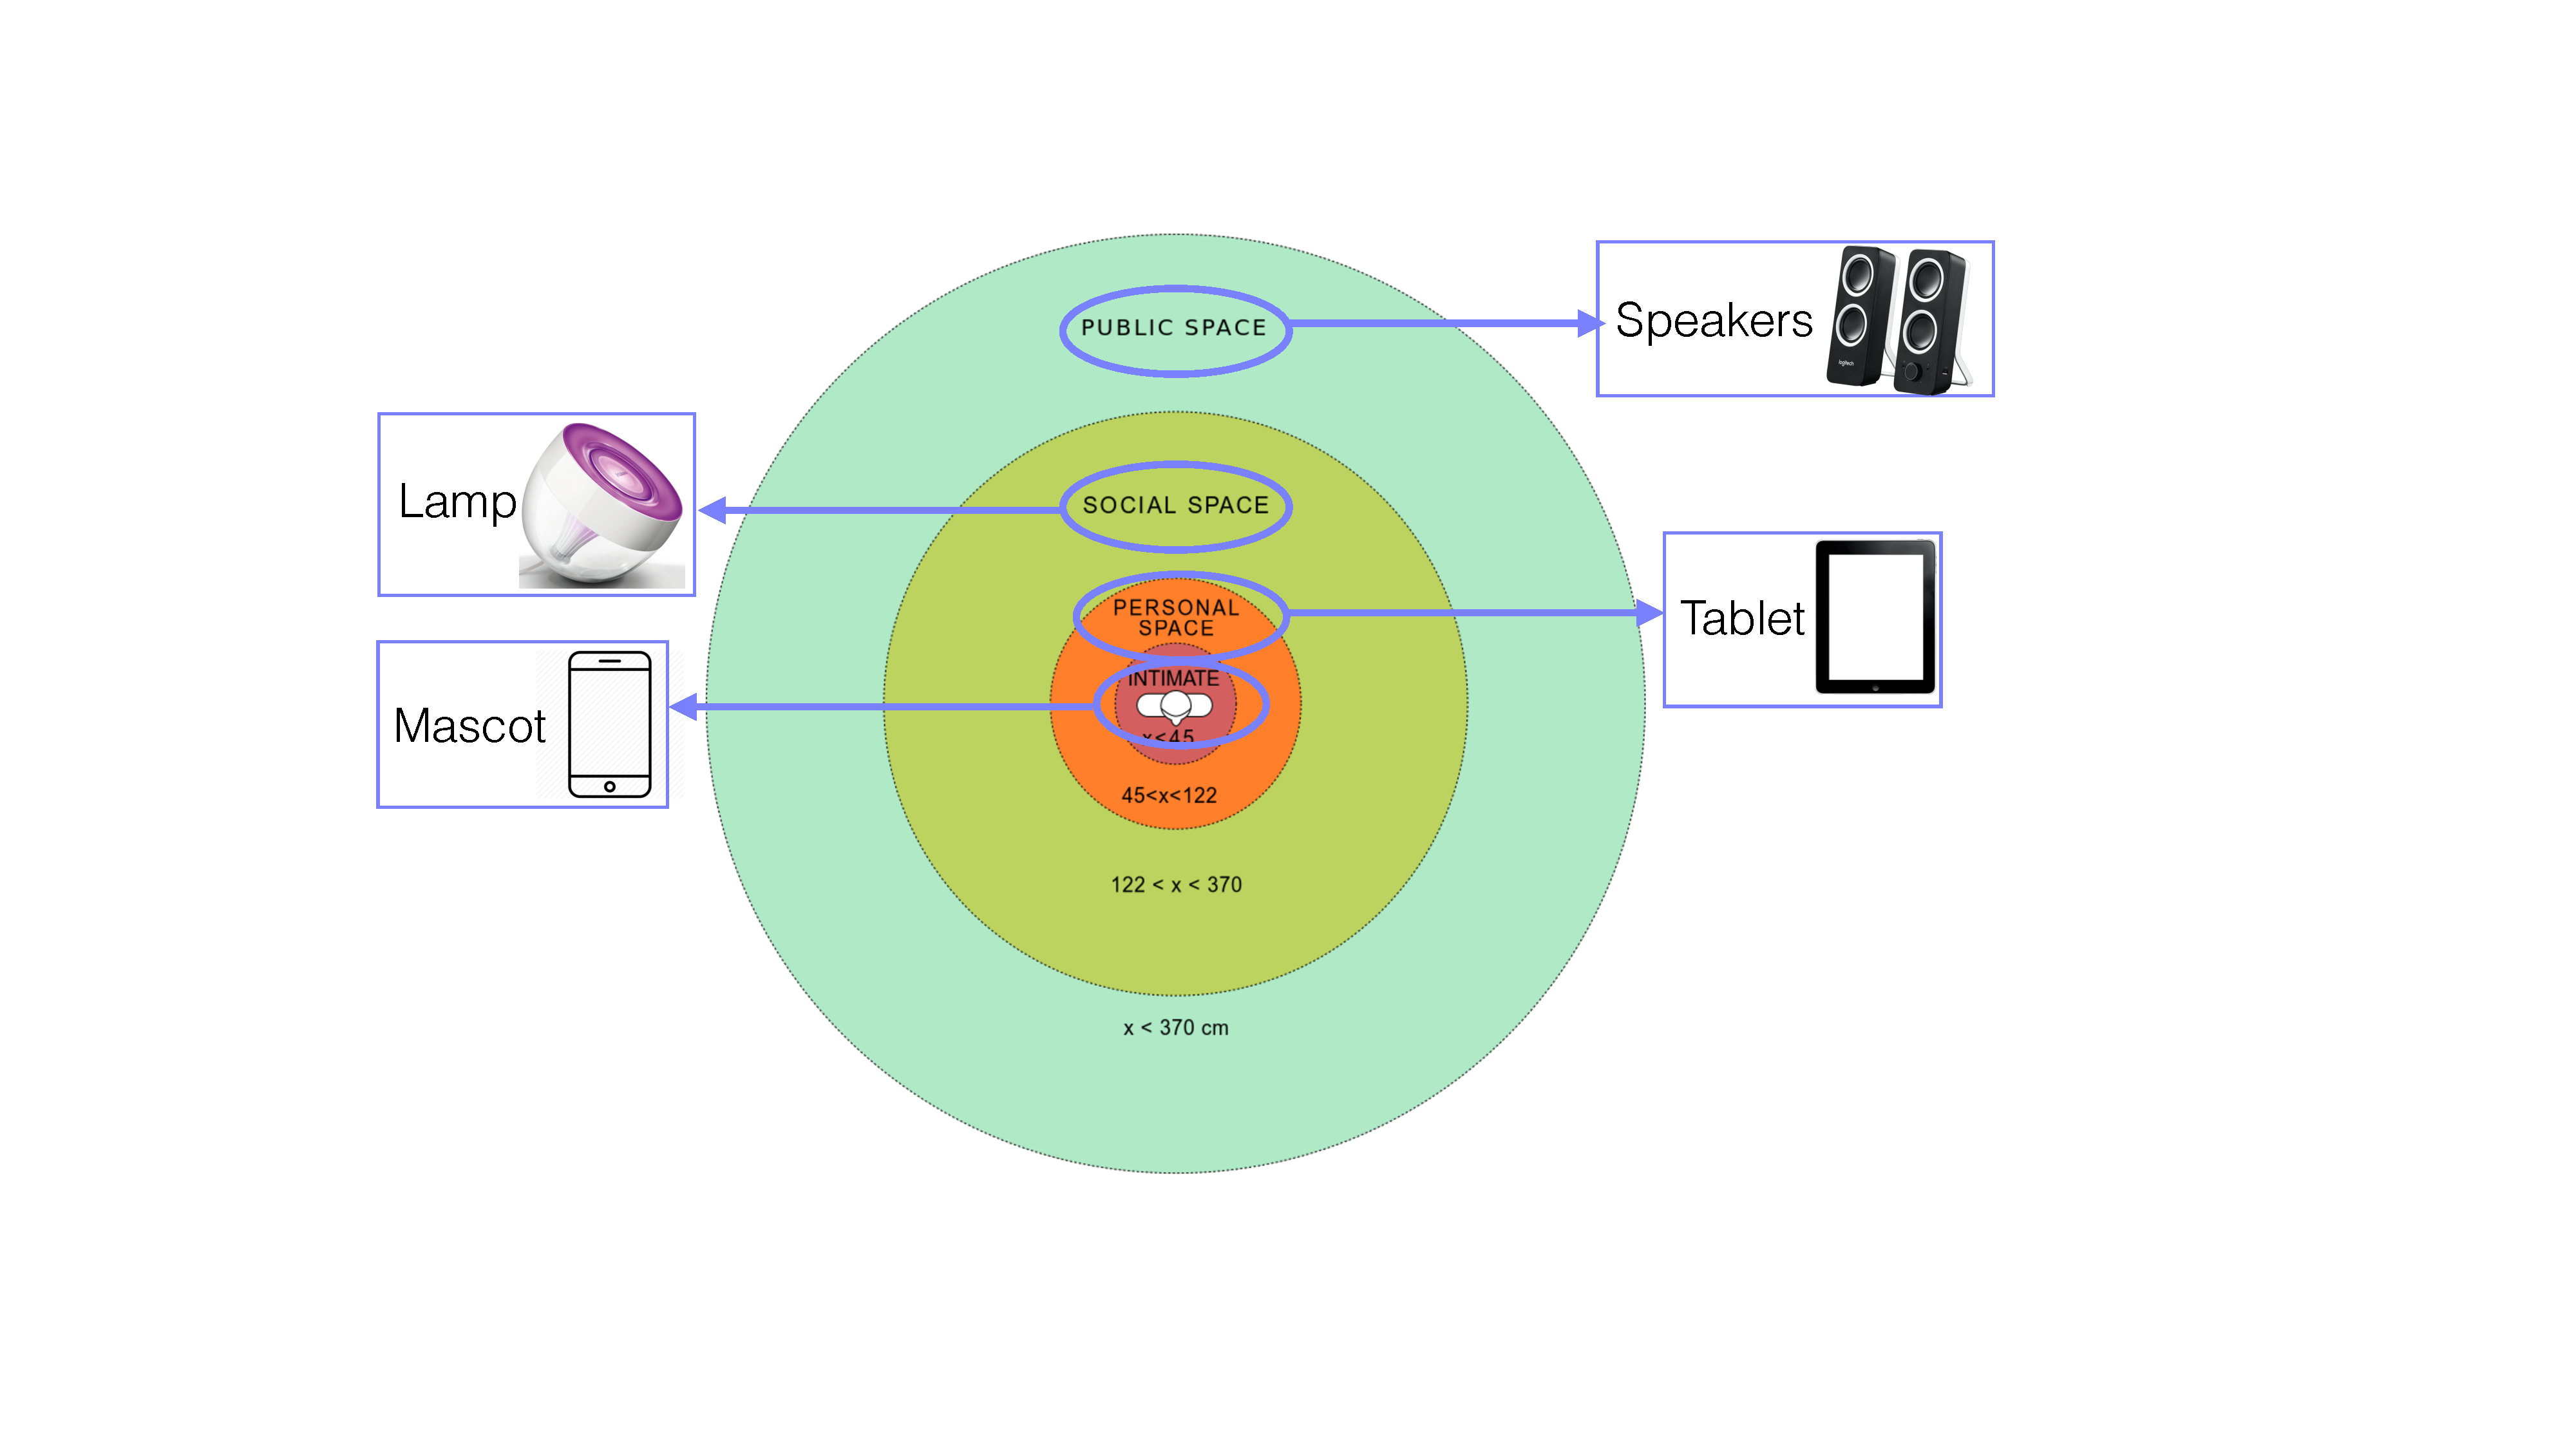
\includegraphics[scale=0.30]{Proxemics.pdf}
    \caption{Visual representation of Procexics Theory~\cite{hall1966hidden, hall1963system} with distances and associated devices selected for
    this study.}
    \label{fig:Proxemics}
\end{figure}

\textbf{Intimate distance} has a very narrow range - up to 45 cm,
and in the context of human-human interaction, this distance used for romantic partners or family members.
Thus, by applying it in the context of a device-device interaction, we can come up with
a device whose functionality is only visible and accessible for their owners such as phone vibration.
In our study, we substitute a phone with a term mascot represented as a ubiquitous personal thing.

\textbf{Personal distance} varied from 45 to 121 cm can be presented by tablet.
In comparison to phone vibration where information is only available for owners,
the size of tablet allows to display information for more members.

\textbf{Social distance} covers from 122 to 370 cm and can be reflected by lighting of the lamp.
Our system contains only one lamp which can be visible for the large number of members.

\textbf{Public distance} ranging for more than 3.7 meters is used for public speaking situations.
In the context of SIoT, we can use speakers as a representative of this distance.
We suppose that the functionality of speakers (i.e music play) will be available for everyone in the room.
In comparison to the visibility of the lamp light which is limited due to the size of the lamp,
speakers with the fixed volume of music play will be available for larger members.

Thus, Proxemics Theory helps us to choose devices, conceptualise their interactions,
come up with case-studies and possible actions that these devices represent.

After identifying case-studies, we apply the concept of personality in the context of
social devices by assigning personality trait to each mascot.
In our system, mascots are dynamic objevts and tablet, lamp and speakers are static devices.
The movements of dynamic devices, interacting with all other
devices effect the environment (i.e the state of interacted devices).
Thus, we assigned a unique personality to each dynamic device which we cover in the following section.

We now can take a closer look at the interaction types of our system represented by each case study:
\begin{itemize}
  \item \textbf{Mascot - mascot} interaction, as mascot approaches another,
        they both start to vibrate where the duration of vibration depends on the personality of approaching mascot.
  \item \textbf{Mascot - tablet} interaction, as mascot goes close to the tablet, the background
        color of a screen starts to change based on the personality of approaching mascot.
   \item \textbf{Mascot - lamp} interaction, as mascot goes close to the lamp,
        the lights start to change their colors based on the personality of approaching mascot.
   \item \textbf{Mascot - speakers} interaction, as mascot approaches speakers,
        it starts to play the genre of music based on the personality of approaching mascot.
\end{itemize}

Each of these interaction types are characterized by actions such as phone vibration,
background screen color change, lighting color transformation and music play.
Since these actions are triggered based on the personality trait of approaching mascot,
we need to associate personalities with more specific actions.
The identification of these action will be described in
Sections~\ref{sec:Identifying the vibration level based on the personality traits},
~\ref{sec:Identifying the music preferences based on the personality traits}
and ~\ref{sec:Identifying the color based on personality traits}.

\section{Identifying personality traits}
\label{sec:Identifying personality traits}

In our system, personality is the primary focus of our investigation and
it is based on the Big Five Personality Models which we briefly described
in the related work Section~\ref{sec:Definition of Personality Traits}.
Costa and McCrae integrated their five factors model with many other personality schemes of that time.
Moreover, their enhanced scheme forms the basis of the "NEO-Personality Inventory-Revised"
which is a widely used measurement scale ~\cite{costa2008revised}.
The NEO-PI-R constitutes five personality traits which we also refer as personality dimensions or domains.
These personality traits are \textbf{O}penness, \textbf{C}onscientiousness,
\textbf{E}xtraversion, \textbf{A}greeableness and \textbf{N}euroticism (also known as  OCEAN Model).
Each of these personality dimensions is composed of six facets which are described in Table~\ref{table:personality}.

\begin{table} [h]
\centering
\begin{tabular}{ | m{8em} | m{25em}| }
\hline
\textbf{Personality Traits} & \textbf{Personality Facets}  \\
\hline
\textbf{O}penness & Fantasy, aesthetics, feelings, actions, ideas, values  \\
\hline 
\textbf{C}onscientiousness & Competence, order, dutifulness, achievement striving, self-discipline, deliberation  \\
\hline 
\textbf{E}xtraversion & Warmth, gregariousness, assertiveness, activity, excitement seeking, positive emotions \\
\hline 
\textbf{A}greeableness & Trust, straightforwardness, altruism, compliance, modesty, tender-mindedness  \\
\hline 
\textbf{N}euroticism & Anxiety, angry hostility, depression, self-consciousness, impulsiveness, vulnerability \\
\hline
\end{tabular}
\caption{Personality facets associated with the five dimensions of the Costa and McCrae five factor model of personality}
\label{table:personality}
\end{table}

In addition, the enhanced scheme of Costa and McCrae (see Table~\ref{table:personality})
helps us in forming questionnaire that we use in our study.
The questionnaire is a Likert scale containing 30 personality facets instead of five personality dimensions.
Participants measured each facet with such device behavior as music, color and vibration level (see Chapter 5).
The questionnaire consists of 30 questions including all six facets of
all five dimensions based on NEO-PI-R measured scale~\cite{costa2008revised}.
The reason of not giving participants five questions consisting of the personality
dimensions as a measurement is the desire to get more detailed feedback from them.
Personality dimension are too broad, and as a result leads to less powerful predictions of behavior~\cite{paunonen2001big}.
Moreover, participants may not be familiar with OCEAN model and giving them the description
of each personality domain might assign them our opinion and might be biased.
In this sense, it would be desirable to have a longer questionnaire which measured traits at both the
domain and facet level to have a better understanding of which features of a trait influence aesthetic preference.
Facets would provide greater descriptive details and a better understanding of the personality in comparison to traits.

In addition, considering human-human interaction, people reflect the mixture of all
these personality traits with a different proportions.
A person who is highly straightforward and modest (facets of agreeableness personality
see Table~\ref{table:personality}) also can have such facets as achieving striving and dutifulness
in different proportions (facets of conscientiousness personality).
Thus, since human personality has a more complex pattern, while
applying this concept to social devices, we decided to simplify it.
That means, If the mascot is assigned agreeable personality, we are planning to consider only this trait,
by making this device, for example, highly trustworthy, and extremely modest and neglecting all other personality traits.

\section{Identifying the vibration level based on the personality traits} 
\label{sec:Identifying the vibration level based on the personality traits}

First, we can consider the case of vibrating mascots, where the vibration level
represents or at least gives a clue about which type of personality the approaching mascot has.
In order to associate the level of vibration with a certain personality trait,
we make an assumption about the vibration being conceptualized as a quality of self-expression
that can be characterized as assertive behaviour.
Depending on the personality of the device, the levels of assertiveness,
which are presented as vibration levels, will differ.
Since we decided to base our theory on the Big Five Personality Model, which, as its name implies, is characterized
by five factors, the vibration levels in our system will vary from one to five (where L1 is scored
as the lowest level of assertiveness and L5 represented as a highly assertive personality).
Subsequent studies~\cite{bagherian2016relationship,kirst2011investigating,ramanaiah1993neo,lefevre1981assertiveness}
investigated the relationship between assertiveness and five personality factors (i.e extraversion, neuroticism,
openness to experience, agreeableness, and conscientiousness).
The consistent findings of the differences in personality traits between assertive and
non-assertive behaviors which are described in these papers can aid in developing our system.

In the following study~\cite{bagherian2016relationship}, authors describe the correlation between
assertiveness and personality traits based on regression analysis.
This analysis together with a correlation coefficient
presented in Table~\ref{table:assertiveness}~\cite{bagherian2016relationship} shows that neuroticism,
extraversion and conscientiousness factors are the main predictors of assertiveness
having a p-value\textless .01 (denoted with asterisks) which indicates the significance of the
relationship between these variables.
The factors of agreeableness and openness to experience have shown
no significant relationship in predicting assertiveness.

\begin{table} [h]
\centering
\begin{tabular}{c c c c c c} 
\\
 \hline \hline
						& \textbf{N} 			&\textbf{E}		&\textbf{O}		&\textbf{A}		&\textbf{C}	\\ [0.5ex]
 \hline
 N 						& 1.000 				&				&				&				&	\\ 
 E 						& -.423** 			&1.000			&				&				&	\\
 O 						& -.047 			&-.001			&1.000			&				&	\\
 A 						& -.253** 			&.351**			&.057			&1.000			&	\\
 C 						& -.356** 			&.387**			&.091			&.0263**		&1.000	\\ [1ex]
 \hline
 \textbf{asseriveness}  		& \textbf{-.253**}		&\textbf{.241**}	&\textbf{-.002}		&\textbf{.064}		&\textbf{.225**}	\\
 \hline \hline
 \end{tabular}
\caption{Correlation Coefficients between personality traits and assertiveness}
 \label{table:assertiveness}
 \end{table}
 
Based on Table~\ref{table:assertiveness}, there is a linear correlation between
extraversion and conscientiousness with assertiveness.
Conversely, the inverse relationship between neuroticism and assertiveness
makes this personality traits the lowest predictor.
In addition, the authors did not find any significant relation between agreeableness and openness with assertiveness.
We considered this table as an example, and the results found in other
works~\cite{kirst2011investigating,ramanaiah1993neo,lefevre1981assertiveness} are
also consistent with the results shown in this table.
On the one hand, the high level of assertiveness and extraversion can be explained
as individuals with this type of personality tend to seek stimulation from the environment
that helps them to assert their opinions without hesitation or to take
the initiative while starting a communication with others.
In the case of conscientiousness, since these individuals are more
concentrated and goal-oriented, they may see assertiveness as a tool to achieve these goals.
A neurotic personality trait, on the other hand, is characterized
by people who are unable to assert or approve themselves and have difficulty in coping with stressful
interpersonal situations which explains why assertiveness and neuroticism are inversely correlated to each other.

However, the relationship between openness and agreeableness personality traits with
assertiveness is more ambiguous, in order to draw a conclusion out of it.
Unfortunately, in many research papers that we studied, the correlation between these
personality types and the level of assertiveness is not significant.
In order to make an assumption about what level of vibration would better characterize
these two personality dimensions, we need to refer to other factors.
For example, in addition to assertiveness, we can also consider which motives or needs these
individuals pursue and therefore, make an assumption based on this additional factor.
The authors of the following papers~\cite{costa1988catalog} studied the relationship between
personality traits and needs and provided us PRF (The Personality Research Form) pattern,
which measures 20 needs that each personality trait may have.
Before we study the PRF pattern, let us examine what are the characteristic features
inherent in these two types of personalities.

In the following book~\cite{matthews2003personality}, openness to experience
personality trait is described as a more open individuals with a deep imagination,
who are always open to new knowledge, to some extent even curious and inquisitive and have wide interests.
Given these characteristics, we can consider the needs and motives that these traits have according to the PRF pattern.
The examination of this pattern may help us to understand how individuals behave in a wide variety of situations.
For example, according to Table~\ref{table:2}, the high score of CH describes that
individuals with openness personality dislike routine and avoid it, readily adapts to changes
in the environment, which show how much they appreciate variety.
The high level of UN scale shows that open individuals want to understand
different areas in order to satisfy intellectual curiosity.
Whereas the low level of HA describes their adventurous side of the personality.
All these scales demonstrate the types of behaviors that openness personality may show to fulfill their needs.
Consequently, we can make an assumption that individuals high in openness
personality trait generally behave in a relatively assertive manner
(i.e they take the initiative, lead discussions) in order to broaden their knowledge.
By relatively, we mean that the level of assertiveness needs to be less than the in
extravert and conscientiousness and more than neuroticism personality since they are the
main predictors of assertiveness and the results have high significant value.
The level of vibration that we can assign to our mascot with this personality trait is L3.
 

\begin{table} [h]
\centering
\begin{tabular}{c c c} 
\\
 \hline \hline
PRF	scores				& \textbf{O} 	&\textbf{A}	\\ [0.5ex] 
 \hline
 Social Recognition (SR)		& -10 		& -19		\\ 
 Defendence (DE)			& -13		& \textbf{-48}	\\
 Succorance (SU)			& \textbf{-34}	& 18			\\
 Affiliation (AF)				& -13  		& 19			\\
 Exhibition (EX)				& 23			& \textbf{-31}	\\
 Play (PL)					& 07			& -06		\\
 Understanding (UN)			& \textbf{64}	& 10			\\
 Change (CH)				& \textbf{60}	& -12		\\
 Sentience (SE)				& \textbf{53}	& 13			\\
 Autonomy (AU)			& \textbf{47}	& -26		\\
 Harmavoidance (HA)		& \textbf{-52}	& \textbf{32}	\\
 Abasement (AB)			& 12			& \textbf{58}	\\
 Nurturance (NU)			& 10			& \textbf{55}	\\
 Dominance (DO)			& \textbf{45}	& \textbf{-46}	\\
 Aggression (AG)			& 14			& \textbf{-68}	\\
 Achievement (AC)			& \textbf{46}	& 02			\\
 Order (OR)				& -25		& -17		\\
 Endurance (EN)			& \textbf{33}	& 15			\\
 Impulsivity (IM)				& 24			& 03			\\
 Desirability (DY)			& 07			& 10			\\ [1ex] 
 \hline \hline		
 \end{tabular}
\caption{Joint Factor Loadings for NEO-PI Factors and PRF Scales}
 \label{table:2}
 \end{table}

Agreeableness is described as a personality trait that is perceived as sympathetic,
kind, warm, generous, helpful, forgiving, friendly, unselfish and gentle personality~\cite{matthews2003personality}.
In addition to this definition, having examined the Table~\ref{table:2} we will
analyze their goals, motives and needs that they fulfill while communicating with others.
For example, this type of personality has a high score in AB, NU, HA and low level
of AG, DO. To summarize, the Table~\ref{table:2} gives us clues that individuals who
are high in agreeable personality like to be modest, tend to be self-effacing,
does not need and want to be the centre of attention.
According to the needs of this personality trait, they can also be interpreted as
being shy individuals who feel tense in the presence of others.
Thus, making plausible for us to assume that, in general, people high in agreeableness
behave less assertive than ones who are low in this personality trait.
This shows that the level of assertiveness that agreeable people have should be
relatively less than who have high openness personality.
The level of vibration that we can assign for this personality trait is L2.

To summarize, the vibration level values that we assigned for each personality traits in our system are the following:
\begin{itemize}
\item L1 is assigned to the mascot with neuroticism personality trait where the
      vibration has the lowest level of amplitude (i.e 100 milliseconds per time).
\item L2 is assigned to agreeableness (i.e 200 milliseconds per time)
\item L3 is assigned to openness to experience (i.e 300 milliseconds per time)
\item L4 is assigned to conscientiousness (i.e 400 milliseconds per time)
\item L5 which represents the highest vibration level and the longest duration
      is assigned to extravert personality trait (i.e 500 milliseconds per time)
\end{itemize}



\section{Identifying the music preferences based on the personality traits}
\label{sec:Identifying the music preferences based on the personality traits}

The next case-study that we consider is the mascot-speakers interaction.
When a person holding a mascot approaches the speakers,
the music starts to play according to the personality of an approaching device.

People use their favourite music as a badge of social identity to share
information about themselves with others ~\cite{boer2011shared,rentfrow2007content}.
Given that they see music as a tool for revealing one’s personality characteristics ~\cite{rentfrow2006message},
in our study, we make the assumption that music can be a good representation of the personality of social devices.

For years researchers have investigated the correlation between genres of the music and personality
traits ~\cite{schafer2009functions,george2007association,zweigenhaft2008re,dunn2012toward}.
However, the genre labels can be biased and subjective, meaning that the user or
participant might have a different understanding of these genres ~\cite{rentfrow2011structure}.
Thus, genre labels might not be able to fully describe someone’s music preference.
The preferences focused on genres are limited in several ways and the authors of the
following paper tried to give a more nuanced assessment of music preferences.

Rentfrow and Gosling ~\cite{rentfrow2003re} were first who provided a categorisation
of musical genre preferences that were not based on exemplary genres but on the musical
characteristics that make the genre within a dimension unique.
They developed a five-factor model of music preferences in terms of the
following orthogonal dimensions: \textbf{M}ellow, \textbf{U}npretentious, \textbf{S}ophisticated,
\textbf{I}ntense, and \textbf{C}ontemporary abbreviated as MUSIC ~\cite{rentfrow2011structure}.
The fact that preferences for each dimensions are independent of the preferences
from the other dimensions makes this model orthogonal.
Before associating these music dimensions with the Big Five personality factors,
we would like to take a close look at other music patterns.

While categorizing music preferences, other authors proposed a different number of music genres and dimensions.
For example, George et al ~\cite{george2007association} studied 30 music styles and revealed eight categories.
Schafer and Sedlmeier ~\cite{schafer2009functions} used 25 genres and found six dimensions.
Whereas, Rentfrow and Gosling decided to arranged 23 styles into five dimensions.
The authors also validated their categories in 3 different studies
using a large sample size which makes this model robust.
Moreover, using the parsimonious number of musical genres is important since otherwise,
it would result in too few studies falling within a single category.
Thus, we expect that the MUSIC model is the most elaborate and robust
multidimensional framework to date for conceptualising and measuring music preferences and personality traits.

We, now, take a close look at each dimension of MUSIC pattern.
The factor analysis of the music preferences from each of three studies proposed five dimensions:
\textbf{m}ellow, \textbf{u}npretentious, \textbf{s}ophisticated, \textbf{i}ntense, and \textbf{c}ontemporary:
\begin{itemize}
\item The first factor features the following attributes: romantic, relaxing, quiet, slow, sad, unaggressive.
      Examples of music genre that might describe this category are smooth jazz, R B/soul, soft rock,
      adult contemporary, electronica, mainstream country and so on.
\item The second factor is described with uncomplicated, soft, acoustic pieces of music and is from new country,
      bluegrass, rock-n-roll, mainstream country, soft rock, religious, pop music genres.
\item The third factor is perceived as inspiring, intelligent, complex, and dynamic including
      avant-grade classic, classical, traditional jazz, world beat, electronica, adult contemporary genres.
\item The fourth factor features loud, aggressive, and not relaxing attributes.
      The music genres that describe this factor are punk, classic rock, heavy metal, and power pop.
\item The fifth factor is defined as not sad, percussive, and electric pieces of
      music and are from rap, R B/soul, europop, electronica genres.
\end{itemize}

Given the description of each of the musical dimensions, we can now correlate them to personality traits.
The scientific predictions or assumptions that we are going to make are based on empirical patterns.
In a review of the following papers, we found a relatively stable relationship between the
above-mentioned MUSIC factors and Big Five
personality ~\cite{schafer2017can,bonneville2013music,fricke2017personality,greenberg2016song,langmeyer2012music}.
The most consistent positive correlation that we have noticed within all these papers was
between openness to experience and Sophisticated dimension.
Meaning that participants who scored high in openness liked
Sophisticated music more than those participants who scored low.
However, one should expect them also show heightened preference for Mellow musical styles.
The next significant relationship that the authors mentioned was the linear correlation between
extraversion and Contemporary which includes rap, R B/soul, europop, electronica music genres.
Agreeableness is correlated with linking for Unpretentious music category.
Comparing the relationship between openness and extraversion and the music categories fits them,
the correlation between agreeableness and its musical dimension is more weak.
Moreover, it was also difficult to find the strong correlations between
conscientiousness and neuroticism personality traits and MUSIC factors which are
also consistent across all above-mentioned studies.
Thus, we are planning to make a weak assumption that individuals with the
conscientiousness and neuroticism are inclined to enjoy Unpretentious and Contemporary music respectively.
In addition, the results across all these papers suggest the negative correlation between
neuroticism and conscientiousness with Intense dimension.
We believe that the knowledge of the negative relationship between these variables will aid us to eliminate
the possibility that participant during experiments might assign this personality traits to this music genre.

To summarise the categories that we decided to assign to each personality trait in our system are the following:
\begin{itemize}
\item Openness to experience will be linked with Sophisticated dimension.
      Meaning that when the mascot with this personality trait will approach the speakers,
      the avant-grade classic, classical, traditional jazz, world beat, electronica, adult
      contemporary music genres will be played.
\item Extraversion which will be linked with Contemporary music will imply that as soon as the extravert
      mascot will come close to the speakers, the rap, R B/soul, europop, electronica music genres will be played.
\item Agreeableness will be linked to the Unpretentious dimension which consists of new country,
      bluegrass, rock-n-roll, mainstream country, soft rock, religious, pop music genres.
\item Conscientiousness will be linked Unpretentious
\item Neuroticism will be linked Contemporary
\end{itemize}

\par Additionally, we assume that assigning a music category to each personality trait,
as opposed to assigning a particular genre, will help participants to broaden the understanding of music preferences.
Therefore, with the help of the arrangement of these genres into categories,
the correlation between personality traits and Music categories will be less varied.
Moreover, in order to help participants to better understand the system and the personality of a mascot,
instead of giving to them a questionnaire with the list of songs and with the genres that they
belong to, our system plays the music from each dimension category.
The main reason for doing that is to measure the personality traits at the right level of specificity.
Zuckerman, Kuhlman, and Camac ~\cite{zuckerman1988lies} pointed out that the level at which one
should evaluate personality characteristics depends on the purposes for which these characteristics are being assessed.
This leads us to the decision to add a context to our experiments.
We expect that participants seeing the mascot affecting the environment
(e.g triggering speakers to play the music), will be able to measure mascots'
personality according to their activities and the change of environment as a result of that behavior.

\section{Identifying the color based on personality traits}
\label{sec:Identifying the color based on personality traits}

In this section we consider two case studies: mascot-lamp and mascot-tablet interactions.
Both of these interaction types are represented by the color change such as
lighting color and background screen color respectively.
The two scenarios that we considered are the following: when a person holding a mascot comes close
to the lamp in first scenario and to the tablet in the second scenario, the lighting
or the screen changes their color according to the personality of approaching mascot.

Before we design the system, it is necessary to understand and clarify the characteristics
of the colors and therefore associate them with a description of the personality traits.
There are many research papers from a variety of disciplines that describe the
relationship between color, behaviors, and personality traits.
For example, Max Lüscher ~\cite{luscher1971luscher} found out the effect of
color preferences on the human behavior which, therefore, may help to determine personality trait.
Herman Cerratto in his work ~\cite{cerrato2012meaning} characterizes colors by
dividing them on their positive and negative aspects.
The following table~\ref{table:color} is adapted from various research
papers ~\cite{luscher1971luscher,cerrato2012meaning,schaie1964color} and
summarizes the characteristics of the colors that we later apply to the design of our system.

\begin{table} [h]
\centering
\begin{tabular}{ | m{8em} | m{25em}| } 
\hline
\textbf{Colors} & \textbf{Affective Aspects}  \\
\hline
Red & energy, strength, attention-seeking, exciting, warm, spontaneous, assertive and confident,
aggression and anger, quick-tempered, ruthless, fearful, intolerant, pain  \\
\hline 
Black & depressing and pessimistic, secretive and withholding, conservative and serious,
sadness and negativity  \\
\hline 
Yellow & cheerful, happy, playful, fun, optimistic, uplifting, illuminating, logical, mental clarity,
aids decision-making, originality, creativity, challenging, academic and analytical, communication of new ideas   \\
\hline 
Orange & warm, sociable, optimistic, enthusiastic, cheerful, adventurous, risk-taking, vibrant,
flamboyant, stimulating to the senses,  self-confident, independent, extroverted and uninhibited,
attention-seeking, encourages to socialize  \\
\hline 
Pink & compassion and understanding, nurturing, warmth, hope, calming, sweetness,
naiveté, innocence and inexperience  \\
\hline
White & innocence, purity, cleanliness, simplicity, self-sufficient, pristine and open, new beginnings  \\
\hline
Turquoise &  communication, clarity of thought, balance and harmony, calmness,
idealism and inspiration, self-expression \\
\hline
Green & growth and vitality, renewal and restoration, self-reliance, reliability,
being tactful, emotionally balanced and calm, practical and down to earth, generous, kind and loyal
with a high moral sense, adaptable and flexible  \\
\hline
Blue &  loyalty, trust and integrity, tactful, caring and concerned, reliability, responsibility,
perseverance, idealistic and orderly, authority, devotion and contemplation, peace and calm \\
\hline
\end{tabular}
\caption{Color meaning}
\label{table:color}
\end{table}

Based on the characteristics describes in Table~\ref{table:personality},
we now can correlate some aspects of colors to Big Five personality dimensions.
For example, according to the following papers ~\cite{alschuler1943easel,schaie1961scaling},
the black color represents intense anxiety, fears, depression, upset, hostility and the red color may
connote facets that varies from happiness, excitement, intense, stimulating to aggression, hate, hostility.
Some of these facets ~\cite{costa1988catalog} belong to the neuroticism personality trait.
Thus, in order to convey the \textbf{neuroticism personality trait}, we decided to apply the
mixture of these two colors which lead us to the dark shade of the red which we refer to as blood-red color.

Herman Cerrato in his paper explains the meaning of turquoise color as a separate color, whereas
all other research papers concentrate on blue and green colors.
Since turquoise is a mixture of pale blue and green colors, we decided to combine
these colors and refer it as turquoise.
Based on the reported aspects of these colors (see Table~\ref{table:color}),
we can associate turquoise with \textbf{conscientiousness personality trait}.
Especially, the characteristics of turquoise color such as clarity of thought,
self-expression, self-sufficiency reported in Table~\ref{table:color} matches the
facets that constitute conscientiousness personality.

Yellow color signifies warmth, creativity, adventures, logic, openness to new
ideas, freedom (see Table~\ref{table:color}).
According to the Max Lüscher, this color refers to one’s desire for development
with which emotions and feeling are associated.
Since openness personality portrays such facets as imagination, adventurousness, intellect, ideas
and so on ~\cite{costa1988catalog}, we assume that the meaning of yellow color matches these facets.
Therefore, we expect yellow color to convey \textbf{openness to experiences personality trait}.

Despite the fact that some characteristics of red color also can connote extraversion personality,
there are also some negative aspects of this color such as aggression, fearfully,
hostility and so on which may also represent neuroticism personality trait.
Thus, we decided to emphasize the negative side of red color by mixing it with black color,
in order to highlight the neurotic personality trait even more.
Meanwhile, for extraversion personality trait we decided to pick orange color.
According to the spectral colors, orange is the color between red and yellow on the spectrum of visible light.
Orange combines the energy of red color and the cheerfulness of yellow ~\cite{cerrato2012meaning}.
Orange color represents optimism, cheerfulness, self-confidence, encouraging
to socialize which constitute the facets of \textbf{extraversion personality trait}.
Thus, by assigning an orange color to our social device, we hope that
participants will interpret our mascot as an extravert.

For \textbf{agreeableness}, we assume that softer shade of pink can convey this personality trait.
Psychologically pink is associated with compassion, understanding, warmth, innocence and calming aspects.
White color also represents innocence, purity, openness in terms of straightforwardness (see Table\ref{table:color}).
The affective aspects of both of these colors constitute the facets of
agreeable personality trait~\cite{costa1988catalog}.
Since white is achromatic and has no hue, we decided to combine
pink and white colors, which lead us to the softer shade of pink color.
Therefore, we hope that pink color (i.e soft pink) connotes agreeableness personality trait.


To summarise the colors that we decided to assign to personality traits in our
mascot-tablet and mascot-lamp interaction are the following:
\begin{itemize}
\item Blood-red color is assigned to the mascot with neuroticism personality trait
\item Turquoise color is assigned to the mascot with conscientiousness personality trait
\item Yellow color is assigned to the mascot with openness personality trait
\item Orange color is assigned to the mascot with extraversion personality trait
\item Pink color is assigned to the mascot with agreeableness personality trait
\end{itemize}

\section{Overview of the system based on the applied concepts.}
\label{sec:overview-of-the-system-based-on-the-applied-concepts.}
In this system, mascot is a dynamic device which effects the state of other
devices and the environment by its location in a space.
The tablet, smart lamps and speakers are static devices with a fixed location.
Since the mascot has an impact on the state of the interacted devices,
the concept of personality is applied to each mascot.
Figure~\ref{fig:ConceptInteraction} shows the interaction between social devices in a system.
\begin{figure}[hbt!]
    \centering
    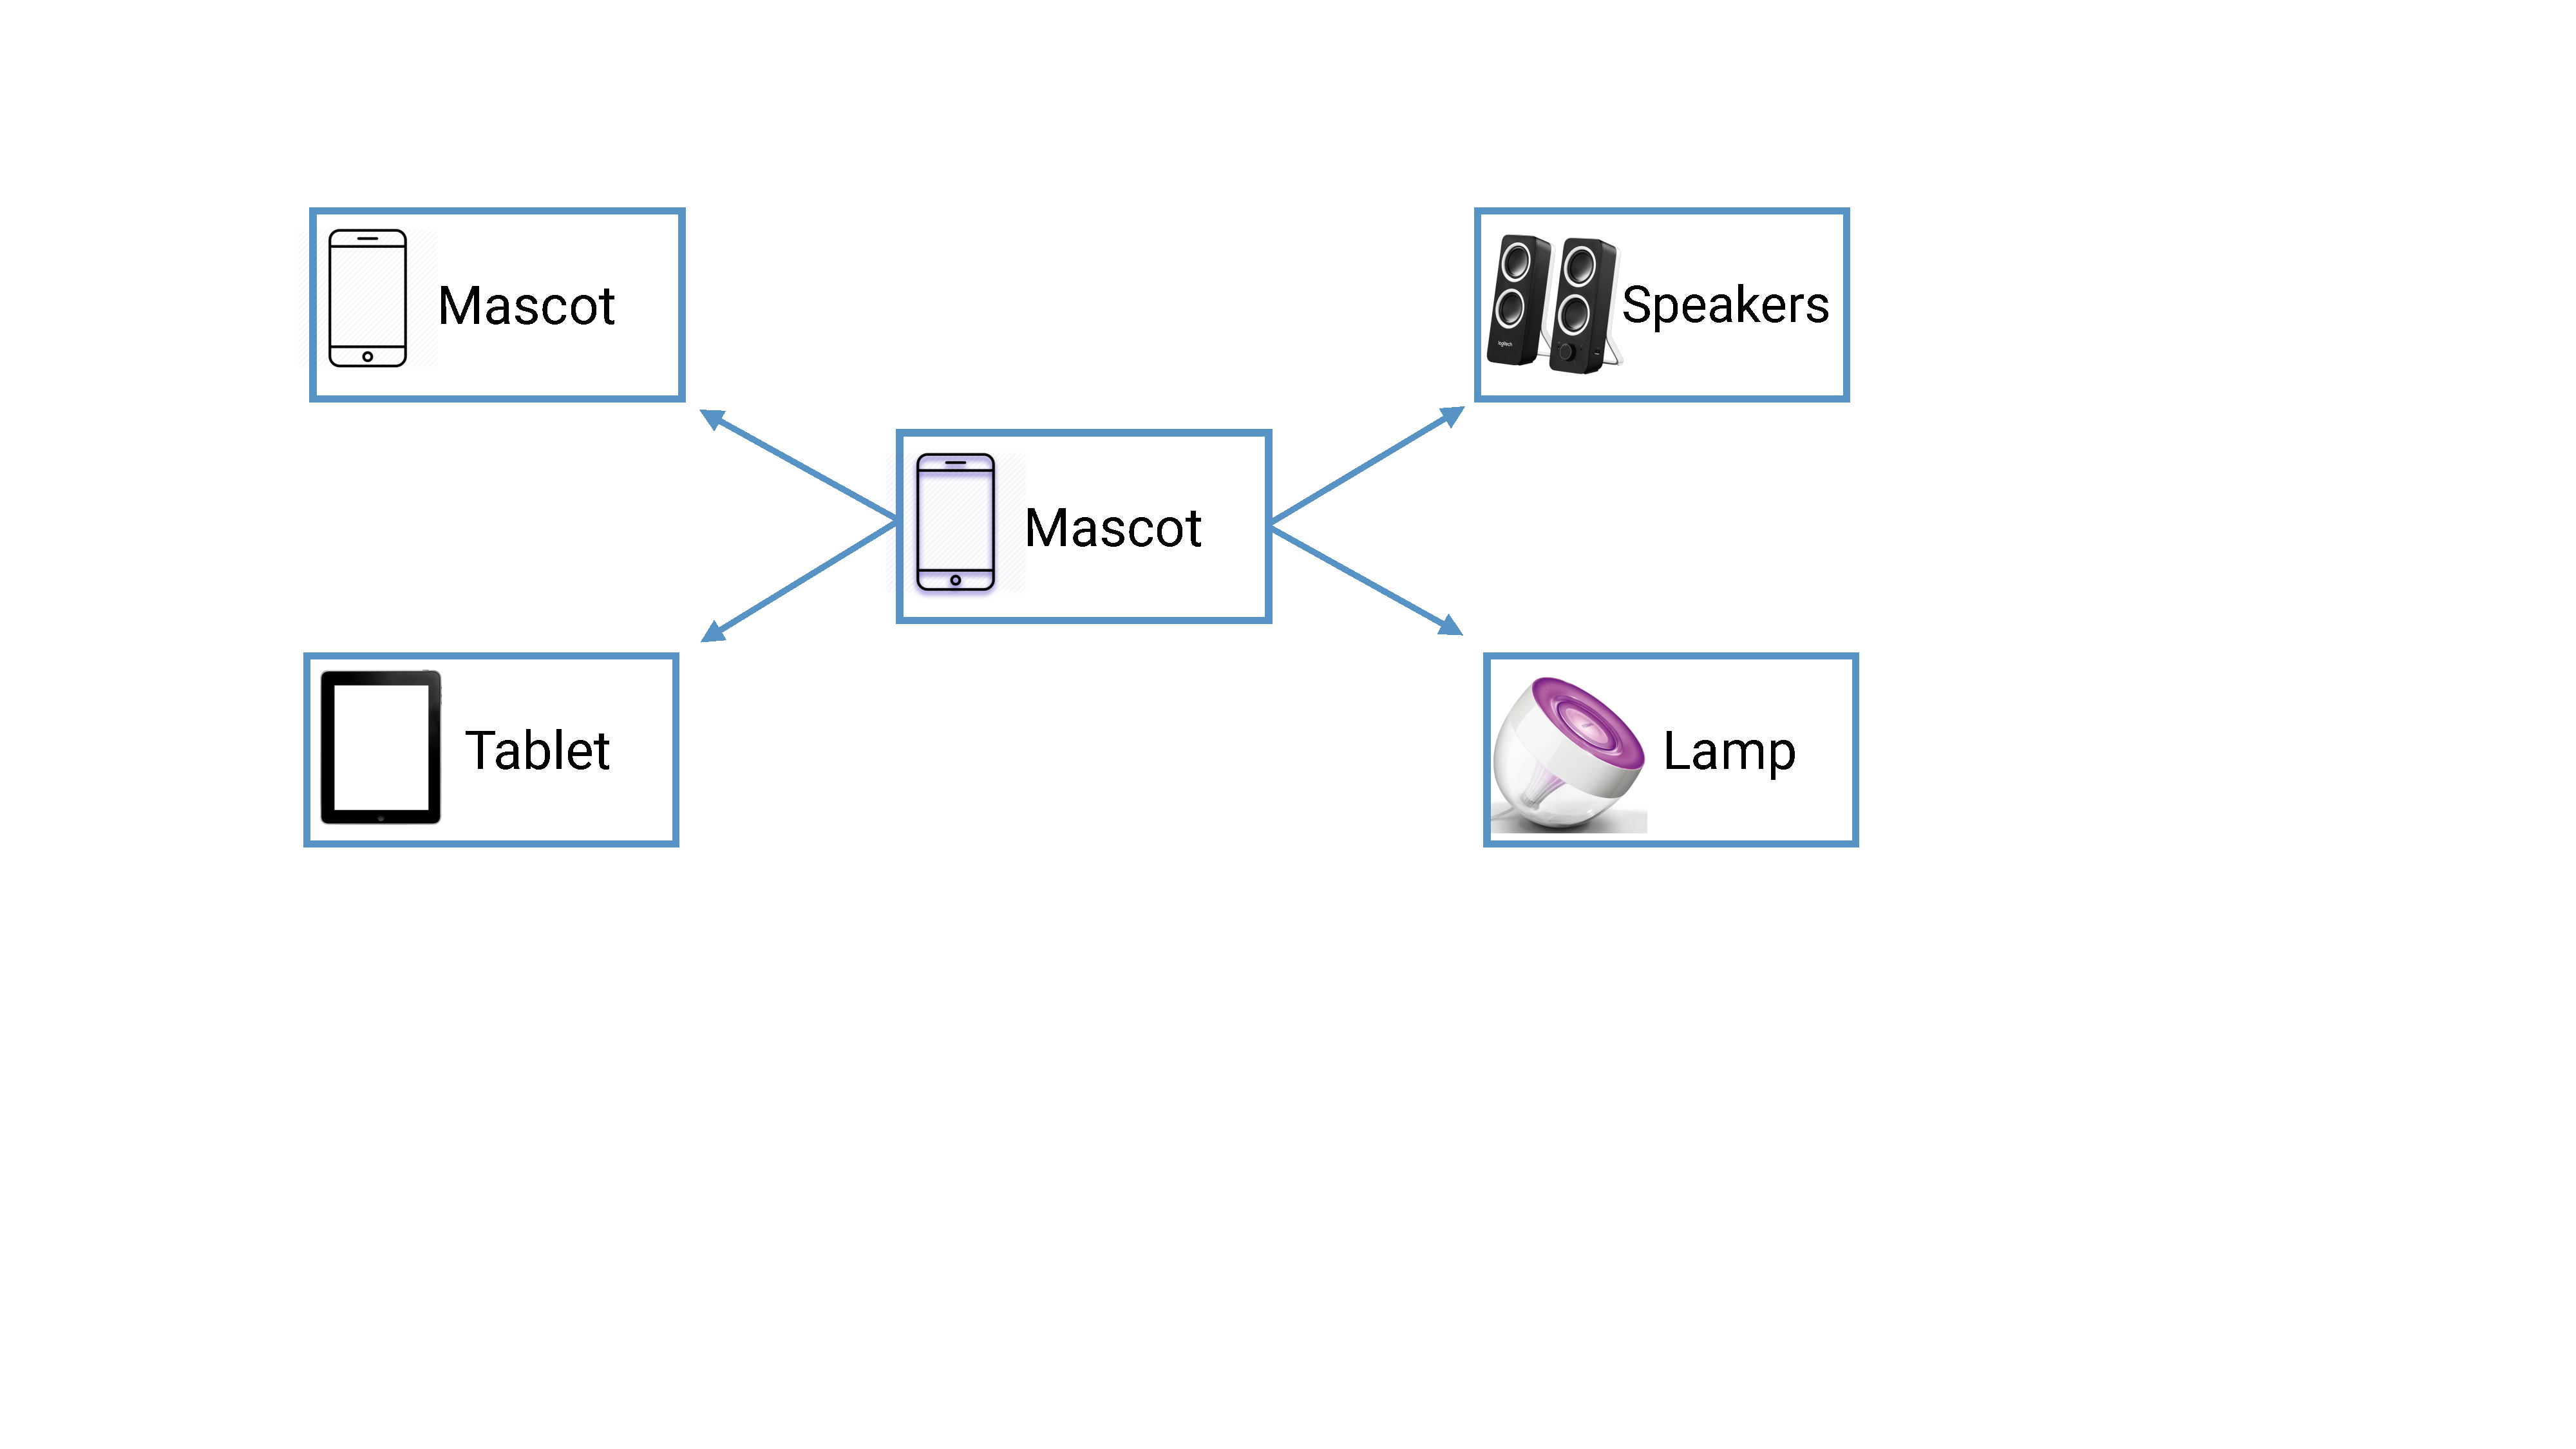
\includegraphics[scale=0.25]{ConceptInteraction.pdf}
    \caption{The visual representation of the interactions between social devices.}
    \label{fig:ConceptInteraction}
\end{figure}

\subsection*{Mascot-mascot interaction.}
When a person holding a mascot comes close to another mascot, they both start to vibrate with
the specific duration of a vibration based on the personality of an approaching mascot.
Figure~\ref{fig:Concept} shows the duration of vibrations in milliseconds associated with
the specific personality traits.

\subsection*{Mascot-speakers interaction.}
When a mascot approaches the speakers, it starts to play a song according to the personality of the approaching mascot.
All types of music are associated with the personality traits described in Figure~\ref{fig:Concept}.

\subsection*{Mascot-lamp and mascot-tablet interactions.}
When a mascot approaches the lamp or a tablet, they change the lighting or screen color according to the
personality of the interacted mascot.
The associations between colors and personality traits are depicted in Figure~\ref{fig:Concept}.

\begin{figure}[hbt!]
    \centering
    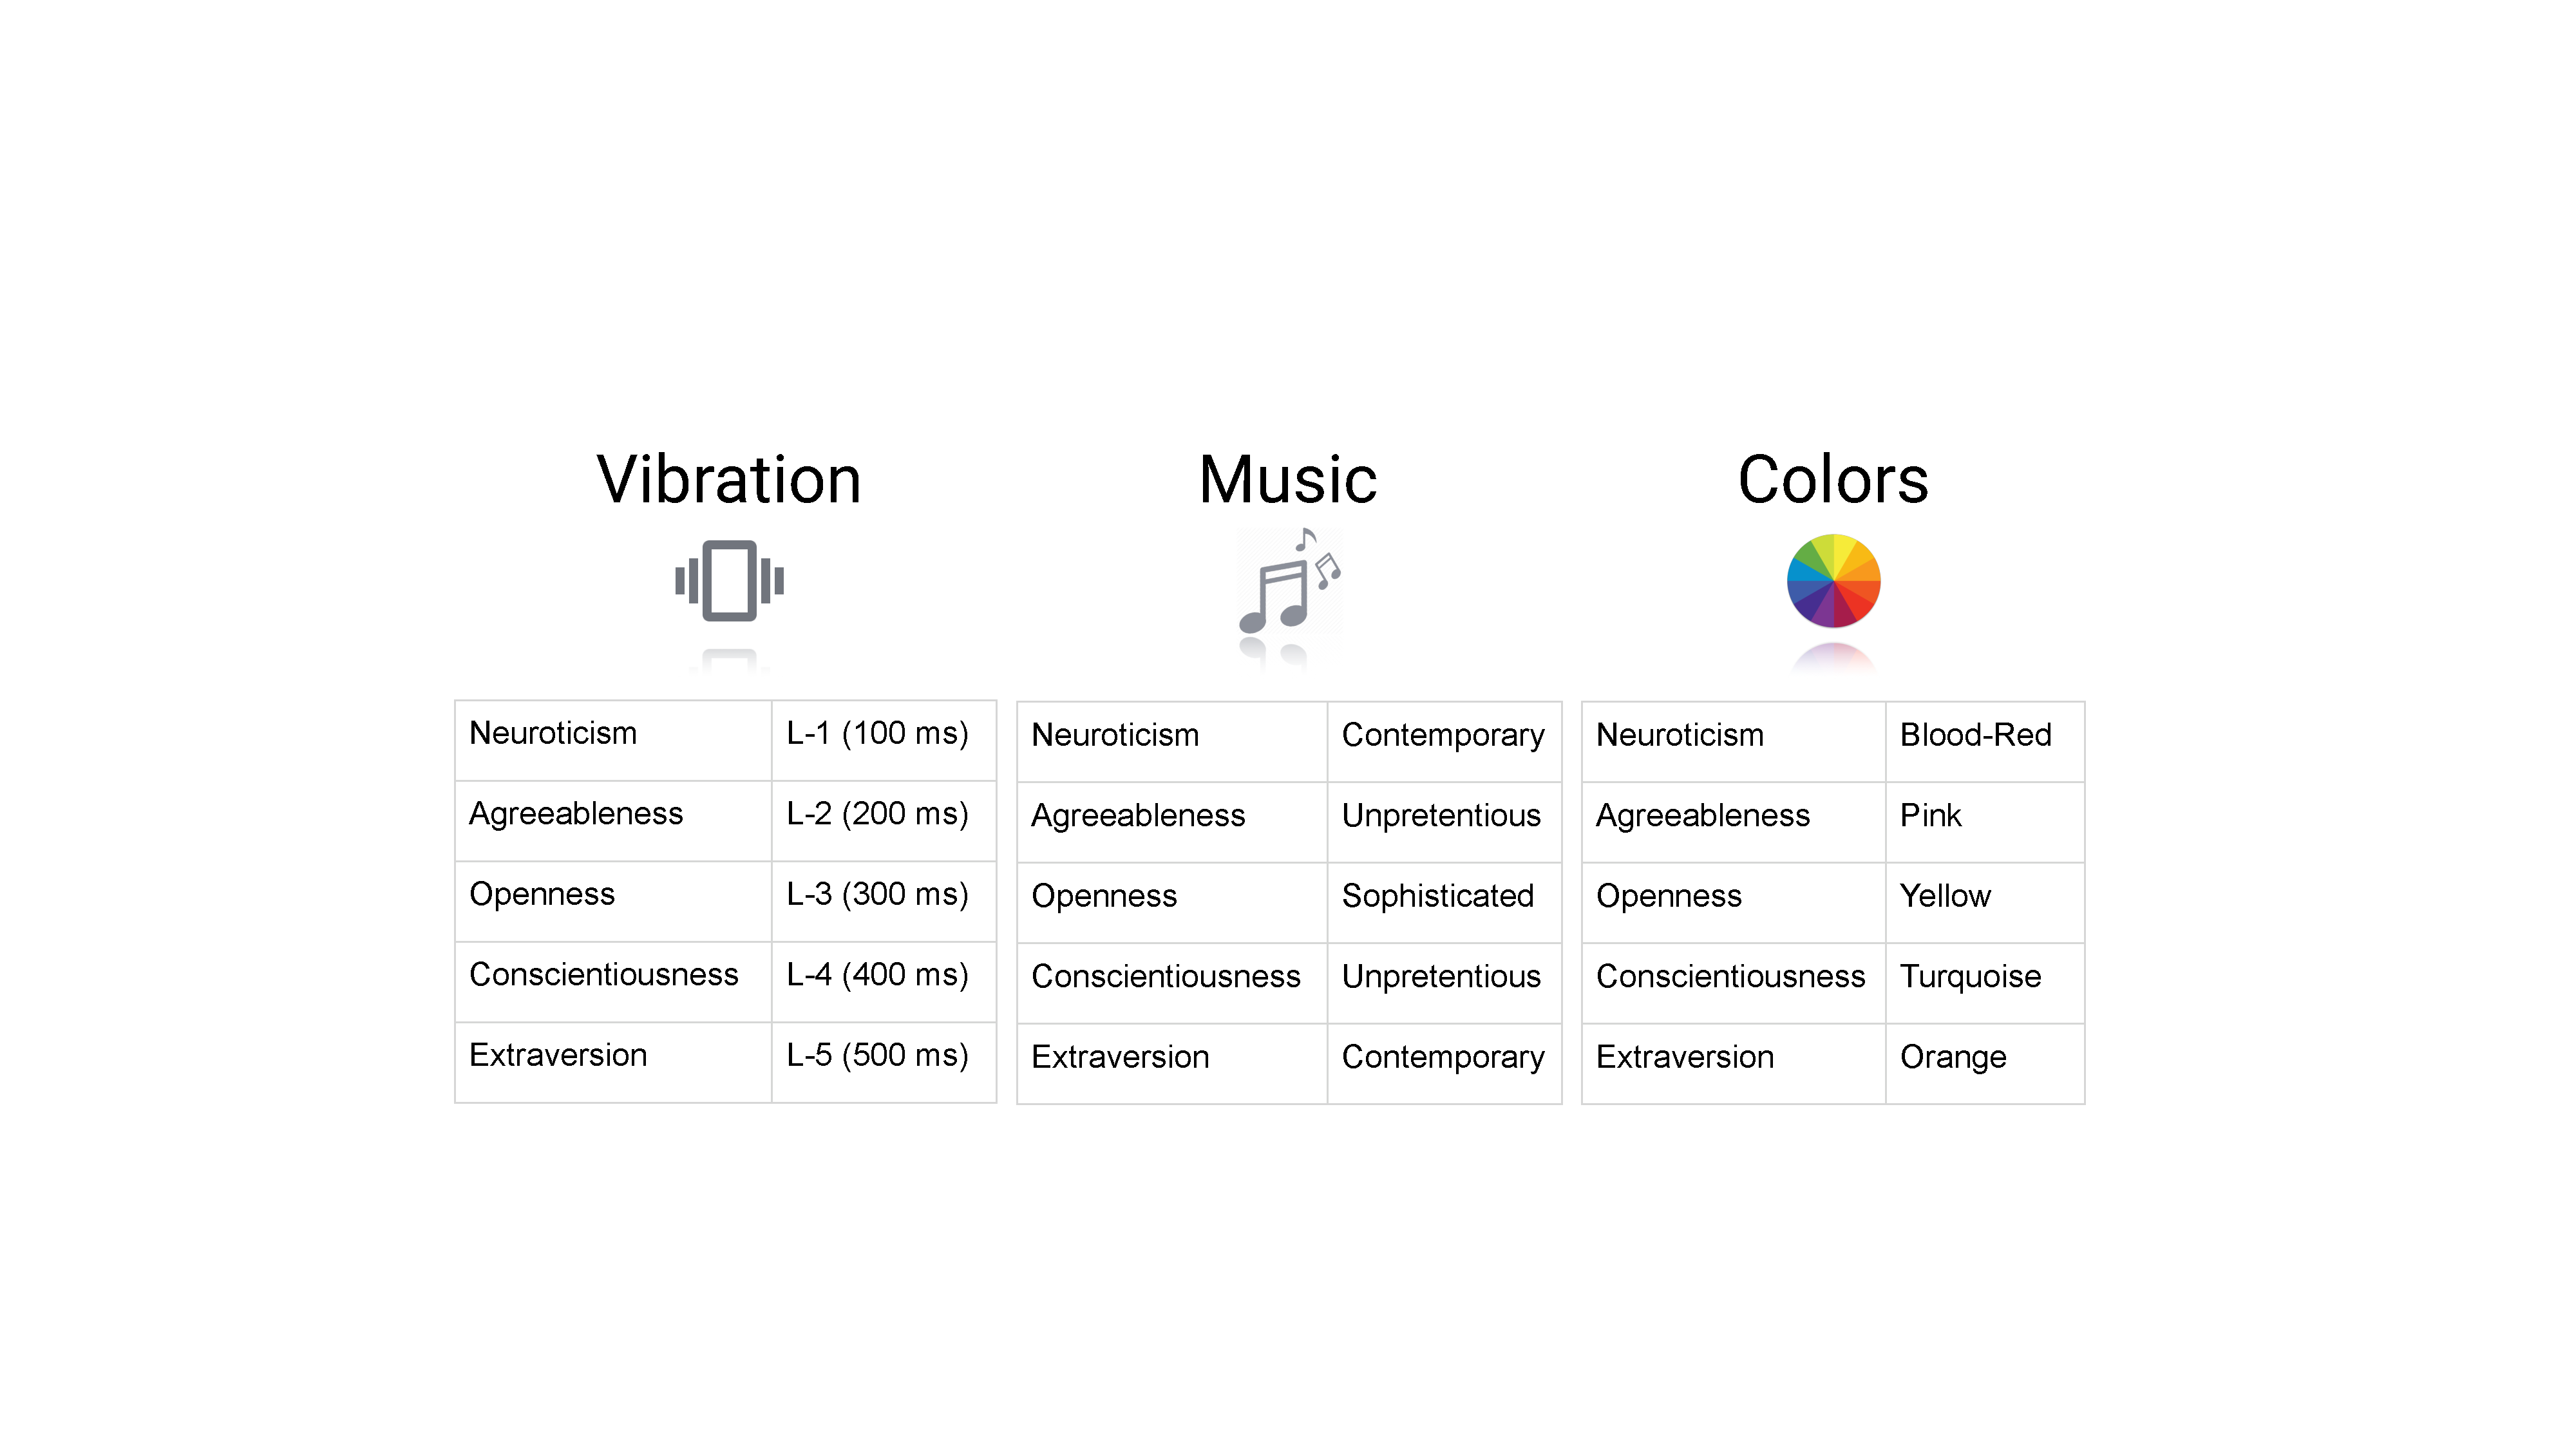
\includegraphics[scale=0.30]{Concept.pdf}
    \caption{The assignment of all personality traits with corresponding actions.}
    \label{fig:Concept}
\end{figure}

Figure~\ref{fig:Concept} is a summary of
all five personality traits with associated actions that we assigned to each mascot.
The assigned personalities with associated actions are used purely for the implementation part in order
to have a consistent system.
In this study, we do not compare the executed system with the user's mental model.
During a user study, we investigated the impact of predefined actions on the way how people
perceive and associate with the personality traits.